\chapter{Multi-Tasking}

\section{Task}
I task rappresentano le azioni da eseguite concorrentemente nel sistema, pianificare dallo Scheduler. 

\begin{itemize}
	\item Dal \textbf{punto di vista del progettista}:
	\begin{itemize}
		\item sono dei moduli software che impegnano il microprocessore per un certo periodo;
		\item permettono di eseguire calcoli e/o azioni di I/O;
		\item possono essere sostituiti, alterati, inibiti o modificati in base alle necessità.
	\end{itemize}
	\item Dal \textbf{punto di vista dell'utente} invece:
	\begin{itemize}
		\item  creano l'illusione di avere un unico sistema monolitico;
		\item  la semplice esistenza e quindi la loro gestione è trasparente all'utente.
	\end{itemize}
\end{itemize}

Per la descrizione del comportamento di ogni task, si è deciso di utilizzare le lambda expression (\ref{sec:lambda}). 

In sintesi i vari task sono istanziati definendo all'interno del \textit{body} del metodo \texttt{init(...)} ogni singolo \textit{behaviour}. Per farlo sono utilizzati: 
\begin{itemize}
	\item i metodi propri del task;
	\item i metodi del Context \ref{sec:context} come mezzo di comunicazione tra i diversi task.
\end{itemize}

Questo ci ha permesso di avere più gradi di libertà nella definizione del comportamento dei task e quindi del codice da eseguire. In quest'ottica non vi è necessità di creare una classe per ogni singolo comportamento, ma basta istanziare due o più volte lo classe e definire diversi body.

\subsubsection{Esempio}
Si vogliono controllare due LED utilizzando il task LedTask; in particolare:
\begin{itemize}
	\item se viene trovato il lucchetto, il led1 viene acceso e il led2 viene spento,
	\item altrimenti, se il lucchetto non viene trovato, il led1 passa a spento e il led2 diventa acceso.
\end{itemize}
\begin{lstlisting}[language=C++]
ledT0 = new LedTask(led1, pContext);
ledT0->init(50, [] {
   	if (pContext->isPadlockDetected()) {
   	  ledT0->led->switchOn();
   	} else {
   	  ledT0->led->switchOff();
	}
});
sched.addTask(ledT0);

ledT1 = new LedTask(led2, pContext);
ledT1->init(50, [] {
   	if (pContext->isPadlockDetected()) {
	  ledT1->led->switchOn();
   	} else {
   	  ledT1->led->switchOff();
	}
});
sched.addTask(ledT1);
\end{lstlisting}

Dopo ogni creazione, ogni task per essere eseguito deve essere aggiunto alla lista di esecuzione dello Scheduler; per farlo si usa \texttt{sched.addTask(<nome del task>)}.

\subsection{Le espressioni Lambda in Wiring/C++11}\label{sec:lambda}
Una \textbf{Lambda expression} (\textit{lambda closure}) è una funzione anonima definita al momento della chiamata. 

Sintassi accettate dal compilatore di Arduino:
\begin{lstlisting}[language=C++]
[ capture-list ] ( params ) { body }
[ capture-list ] { body } 
\end{lstlisting}

\subsubsection{Caratteristiche}
\begin{itemize}
	\item La \textit{capture list} è la lista di variabili che è possibile utilizzare oltre agli argomenti della funzione.
	\begin{itemize}
		\item Se si definisce \texttt{[\&]}, tutte le variabili locali saranno passate per riferimento.
		\item Se non viene specificato niente, la \textit{lambda function} non ha variabili come argomenti e viene indicata con \texttt{[]};
	\end{itemize}
	\item Il tipo di ritorno è \texttt{void}, a meno che non viene specificato diversamente;
	\item Il body della funzione che si trova tra parentesi graffe rappresenta le azioni che devono essere eseguite.
\end{itemize}

\subsubsection{Vantaggi}
\begin{itemize}
	\item è possibile creare una classe "generica" che può avere più istante a cui assegnare più behaviour;
	\item si evita di dover creare per ogni comportamento una classe specifica;
	\item codice modulare, (diverse istanze dello stesso oggetto possono avere diversi body);
	\item definizione del comportamento direttamente dal file \texttt{*.ino}.
\end{itemize}

\subsubsection{Contro}
Per utilizzare le lambda expression siamo stati costretti a rinunciare parzialmente all'\textit{information hiding} della programmazione OO. Questo vincolo è legato al fatto che non è stato possibile passare oggetti come parametro di chiusura.

L'unico modo per passare gli oggetti e quindi i metodi all'interno di queste particolari funzioni è stato mettere tutto \texttt{public}.

\subsection{Generalizzazione del funzionamento di un task}
\begin{figure}[!ht]
	\centering
	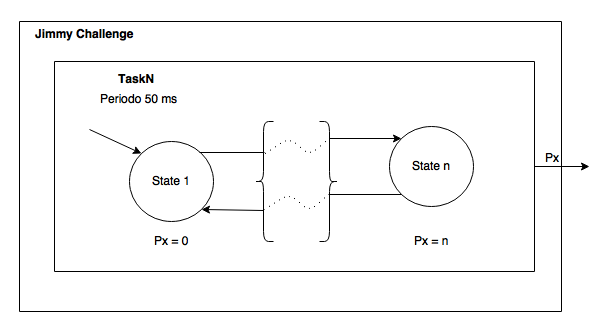
\includegraphics[scale=.60]{img/task_generic.png}
	\caption{Generalizzazione dei task}
\end{figure}

\subsubsection{Elenco dei Task sviluppati:}
\begin{enumerate}
	\item SonarTask
	\item ButtonTask
	\item BuzzerTask
	\item LedTask
	\item LedPwmTask
	\item LedRgbTask
\end{enumerate}

\subsection{SonarTask}
È il task più importante del progetto in quanto:
\begin{itemize}
	\item permette l'interazione utente-sistema sfruttando il sensore ad ultrasuoni;
	\item aggiorna la \texttt{currentDistance} del Context (\ref{sec:context});
	\item in modo indiretto può variare l'evoluzione del sistema
\end{itemize}
Nella classe SonarTask viene definito il metodo \texttt{privare playLevel()} in cui:
\begin{itemize}
	\item si legge la currentDistance dal sonar;
	\item si setta tale currentDistance nel Context;
	\item si gestiscono gli \texttt{status} da inviare alla seriale
\end{itemize}

Dal Context:
\begin{itemize}
	\item si riceve il \textbf{numero segreto} (il lucchetto, cioè la distanza dal sensore)
	\item si riceve il \textbf{delta} (intervallo superiore/inferiore a partire dal lucchetto)
	\item si riceve il \textbf{livello attuale} a cui si sta giocando
	\item si controlla se il lucchetto è aperto con \texttt{pContext->isPadLockOpen()}
\end{itemize}
Sul Context:
\begin{itemize}
	\item se il lucchetto è stato aperto si crea un nuovo livello con \texttt{pContext->setNewLevel()};
	\item se il padLock non è stato completamente sbloccato viene settato come chiuso con \texttt{pContext->setPadlockOpen(false)};
	\item se il padLock non è stato completamente sbloccato viene resettato lo stato di scasso con \texttt{pContext->setLockpicking(false)};
	\item in base al tempo passato nello scassinare il lucchetto (e quindi allo \texttt{status} in cui ci si trova), viene settato \texttt{pContex->setDangerLevel(...)} con un numero da 0 a 4, (che nel LedRgbTask indica il colore da visualizzare sul LED RGB).
\end{itemize}

\begin{lstlisting}[language=C++]
void SonarTask::playLevel() {
	currentDistance = sonar->readDistance();
	pContext->setCurrentDistance(currentDistance);
	int secretDistance = pContext->getSecret();
	int currentLevel = pContext->getLevel();
	uint8_t delta = pContext->getDelta();
	int status = 0;
	int feedbackDistance = 0;
	
	feedbackDistance = abs(currentDistance - secretDistance);
	if (feedbackDistance == 0)
		feedbackDistance = 0;
	else if (currentDistance == 0)
		feedbackDistance = 100;
	
	if(currentDistance <= (secretDistance + delta)
	&& currentDistance >= (secretDistance - delta)) {
		pContext->setPadlockDetected(true);
		timeFound = (millis()/1000) - timeOut;     // inizializzazione a zero
		switch (timeFound) {
			case 0:
			if (pContext->isPadlockOpen()) {
				msgService.sendMsg("Lucchetto livello " + String(currentLevel) + " APERTO", F("all"));
				pContext->setNewLevel();
				if (!pContext->isGameOver()) {
					status = 300 + currentLevel + 1;
					pContext->setPadlockOpen(false);
					pContext->setLockpicking(false);
				}
			} else
			status = 101;
			break;
			case 1:
			status = 101;
			break;
			case 2:
			status = 102;
			break;
			case 3:
			status = 103;
			break;
			case 4:
			status = 104;
			pContext->setDangerLevel(0);
			pContext->setLockpicking(true);
			break;
			case 5:
			status = 104;
			pContext->setDangerLevel(0);
			break;
			case 6:
			status = 105;
			pContext->setDangerLevel(1);
			pContext->setPadlockOpen(true);
			break;
			case 7:
			status = 201;
			pContext->setDangerLevel(1);
			break;
			case 8:
			status = 202;
			pContext->setDangerLevel(2);
			break;
			case 9:
			status = 203;
			pContext->setDangerLevel(3);
			break;
			case 10:
			status = 204;
			pContext->setDangerLevel(4);
			pContext->setPadlockOpen(false);
			break;
			case 11:
			status = 205;
			pContext->setDangerLevel(4);
			break;
		}
	} else {
	timeOut = millis()/1000;
	pContext->setPadlockDetected(false);
	pContext->setLockpicking(false);
}
msgService.sendInfo(currentDistance, status, currentLevel, F("remote"));
}
\end{lstlisting}

Per la rilevazione della distanza della mano dal sensore è stata utilizzata la libreria \textbf{NewPing} \ref{sec:newping}.

\subsubsection{\underline{Libreria \href{http://playground.arduino.cc/Code/NewPing}{NewPing}}}\label{sec:newping}
\textbf{Caratteristiche}
\begin{itemize}
	\item Funziona con diversi modelli di sensori ad ultrasuoni: SR04, SRF05, SRF06, DYP-ME007 e Parallax Ping™;
	\item Non ha un \textbf{lag} di un secondo se non si riceve un ping di eco
	\item Ping coerente e affidabile fino a 30 volte al secondo.
	\item Timer interrupt method per sketch event-driven
	\item Metodo di filtro digitale Built-in \texttt{ping\_median()} per facilitare la correzione degli errori.
	\item Utilizzo dei registri delle porte durante l'accesso ai pin per avere un'esecuzione più veloce e dimensioni del codice ridotte.
	\item Consente l'impostazione di una massima distanza di lettura del ping "in chiaro".
	\item Facilita l'utilizzo di più sensori.
	\item Calcolo distanza preciso, in centimetri, pollici e uS.
	\item Non fa uso di \texttt{pulseIn}, in quanto lento e con alcuni modelli di sensore a ultrasuoni restituisce risultati errati.
	\item Attualmente in sviluppo, con caratteristiche che vengono aggiunte e bug/issues affrontati.
\end{itemize}


\subsection{ButtonTask}
Questo task controlla se è avvenuta la pressione del \textit{button}.
Finché il gioco non è finito è possibile stampare su terminale un messaggio che indica la posizione del lucchetto. 

Se il gioco è finito, ma il bottone viene comunque premuto, si avvia una divertente \textbf{\textit{easter egg}} legata al BuzzerTask e ad un famoso gioco degli anni '80\dots


\subsection{BuzzerTask}
Questo task controlla i suoni che il \textit{buzzer} deve emettere attraverso il metodo \texttt{buzzerT0->buzzer->playSound(<num>)}

\begin{itemize}
	\item Se il gioco non è finito e il lucchetto non è ancora stato trovato, viene emesso il suono 0;
	\item Se il gioco non è finito e il lucchetto è stato trovato, viene emesso il suono 1;
	\item Se il gioco è finito e il pulsante premuto, viene emesso il suono 2 (\textbf{\textit{easter egg}}).
\end{itemize}

\subsection{LedTask}
Questo task controlla l'accensione e lo spegnimento del LED verde.

\begin{itemize}
	\item Se il gioco non è finito e il lucchetto è stato trovato, il LED viene acceso;
	\item Se il gioco non è finito e il lucchetto non è ancora stato trovato, il LED viene spento.
\end{itemize}

\subsection{LedPwmTask}
Questo task gestisce il LED verde utilizzando il pin PWM grazie ai seguenti metodi:
\begin{itemize}
	\item \texttt{ledPwmT0->ledPwm->setIntensity(<num>)} per gestire l'intensità luminosa (anche temporizzata) del LED;
	\item \texttt{ledPwmT0->ledPwm->switchOff()} per spegnere immediatamente il LED.
\end{itemize}
\begin{itemize}
	\item Se il lucchetto non è stato aperto e non è stato trovato, si aumenta l'intensità del LED usando un ciclo for inizializzato a 64 (in modo da non partire dal LED completamente spento) per arrivare a 255 (valore massimo consentito).
\end{itemize}

\subsection{LedRgbTask}


\section{Scheduler}

\section{Context}\label{sec:context}




